% -*- TeX -*- -*- UK -*- -*- Soft -*-

\chapter{Python and Jupyter Code}
\label{sec:PythonandJupyterCode}

Prepared by CJ Willers.


\section{Code Supplement to Chapter~4}
\label{sec:CodeSupplementtoChapter4}



The repository that contains the \LaTeX{} source code has a Jupyter notebook with interactive plotting widgets, see \lstinline{code/chapter4-graphics.ipynb}.

\subsection{Visualising Weight and Bias Effects}
\label{sec:VisualisingWeightandBiasEffects}

Equation~\ref{eq:c01-03-sigmoidfunction} and following code shows how the neuron weight and bias affects the sigmoid output.

\begin{lstlisting}
x = np.linspace(0,1,300)
p = ryplot.Plotter(1,4,4,figsize=(15,15),doWarning=False)
ws = [5,10,20,40]
bs = [-20,-10,-5,-2]
for iw,w in enumerate(ws):
    for ib,b in enumerate(bs):
        y = sigmoid(x,w,b )
        p.plot(1+ib+iw*len(bs), x, y, f'w={w} b={b}',maxNX=1,maxNY=1,xAxisFmt='%.0f',yAxisFmt='%.0f',pltaxis=[0,1,0,1] )
\end{lstlisting}

{\centering 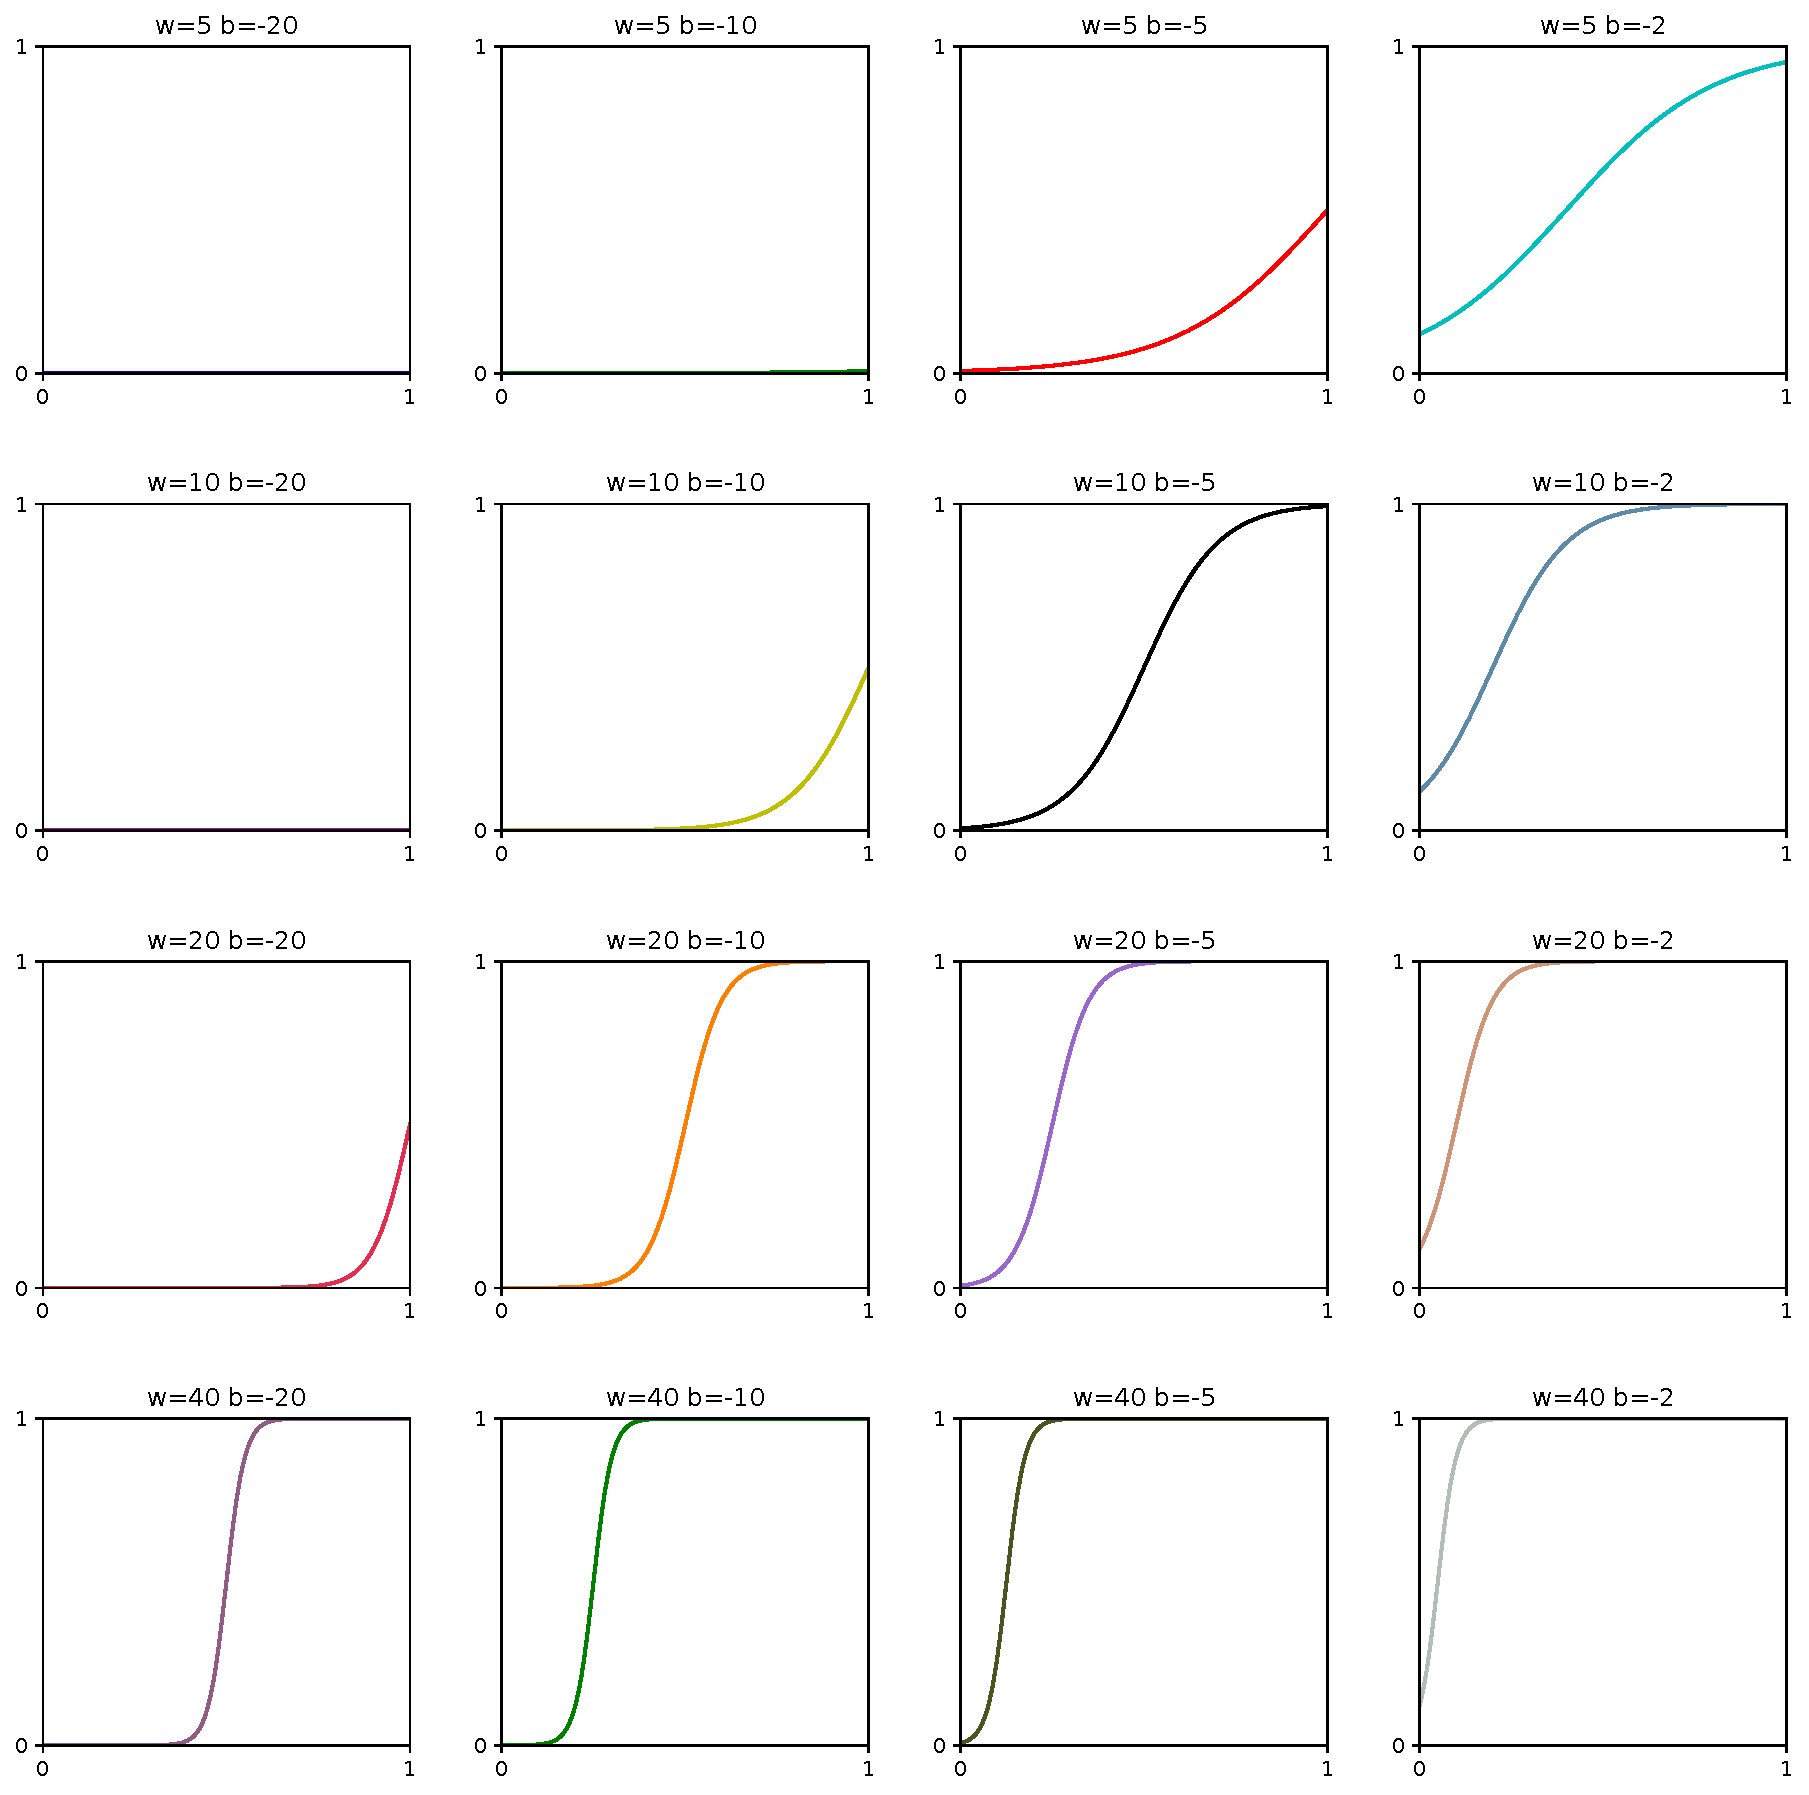
\includegraphics[width=\textwidth,]{eps/sigmoid4x4plot} \par}

Observe how the output (vertical axis) changes as $w$ changes (downward in the set of graphs).


\subsection{Approximating Functions with Neural Nets}
\label{sec:ApproximatingFunctionswithNeuralNets}

The following Python code provides slider functions in a Jupyter notebook, providing similar functionality to the interactive graphics on the web site.  Open a Jupyter notebook or lab book and enter and play with the code.  See the code for comments.

\begin{lstlisting}[language=Python]
import numpy as np
import matplotlib.pyplot as plt

%matplotlib inline


def sigmoid(x,w,b):
    return 1 / (1 + np.exp(- x * w - b))
    

def plot_activation_sh(**kwargs):
    """Plot the activation of a single output neuron from a set of hidden neurons,
    given a list of s values (hidden neuron bias/weight)
    and a list of h values (output neuron weight for each hidden neuron).
    
    The list has a 1.5 x number of hidden neurons tuples.
    Each tuple defines one slider, in terms of its name, default value and lo/hi limits.
    
    Each pair of two hidden neurons (with different s-values) share one h-weight value.
    The two s-values define the lower and upper s-values, defining an interval on the x axis.
    The output of the two s-value neurons are subtracted and multiplied with the h-weight value.
    This set of three values (2xs and 1xh) defines one 'pulse' along the x-axis with height h.
    
    The network parameters are given as **kwargs, on the following understanding:
    1) tuples with s values (one tuple for each hidden neuron input weight, s=bias/weight)
    2) tuples with h values (one tuple shared between each pair of two hidden neurons)
    """
    numNeuronPairs = int(len(kwargs)/3)
    x = np.linspace(-1,1,300)
    wh = 300
    sum = 0
    for i in range(numNeuronPairs):
        lonum = f'{i*2+0:02d}'
        hinum = f'{i*2+1:02d}'
        sum += kwargs[f'h{lonum}-{hinum}'] * sigmoid(x,wh,-kwargs[f's{lonum}']*wh) - \
            kwargs[f'h{lonum}-{hinum}'] * sigmoid(x,wh,-kwargs[f's{hinum}']*wh) 
    svals = [kwargs[f's{s:02d}'] for s in range(2*numNeuronPairs)]
    fig, ax = plt.subplots(figsize=(8, 6))
    ax.set_xlabel('x')
    ax.set_ylabel('y')
    ax.plot(x, sum,  linewidth=2)
    ax.set_ylim(np.min(sum),np.max(sum))
    ax.set_xlim(min(svals),max(svals))

    
def setupShow_sh(ss,hs,hidden=False,step=0.01):
    """Load tuples and set up the sliders.
    
    ss: list of s-value tuples
    hs: list of h-value tuples
    hidden: if True don't display sliders
    step: slider step values
    
    """
    sliders = []
    for i,(lo,hi,val) in enumerate(ss):
        slid = widgets.FloatSlider(value=val,min=lo,max=hi,step=step,
                            description=f's{i:02d}',disabled=False,continuous_update=False,
                            orientation='horizontal',readout=True,readout_format='.2f')
        if hidden==True:
            slid.layout.display = 'none'
        sliders.append(slid)

    for i,(lo,hi,val) in enumerate(hs):
        slid = widgets.FloatSlider(value=val,min=lo,max=hi,step=step,
                            description=f'h{2*i:02d}-{2*i+1:02d}',disabled=False,
                            continuous_update=False,orientation='horizontal',
                            readout=True,readout_format='.2f')
        if hidden==True:
            slid.layout.display = 'none'
        sliders.append(slid)

    kwargs = {slider.description:slider for i,slider in enumerate(sliders)}
    interact(plot_activation_sh,**kwargs);

    
# ss is a list of slider s-values (min, max, value)
# hs is a list of slider h-values (min, max, value)
case = 1
if case==0:
    ss = [(-1, 1,-0.9),(-1, 1,-0.71), (-1, 1,0.01), (-1, 1,0.36)]
    hs = [(-2, 2, 0.69),(-2, 2, -1.52)]
    hidden = False
elif case==1:
    ss = [(-1, 1,0),(-1, 1,0.2), (-1, 1,0.2), (-1, 1,0.4), (-1, 1,0.4), (-1, 1,0.6), 
          (-1, 1,0.6), (-1, 1,0.8), (-1, 1,0.8), (-1, 1,1)]
    hs = [(-2, 2, 0.3),(-2, 2, -1.0),(-2, 2, 0.2),(-2, 2, -1.2),(-2, 2, -0.3)]
    hidden = True

setupShow_sh(ss,hs,hidden=hidden)    
\end{lstlisting}

The Jupyter notebook should display the sliders (if not hidden) and the reconstructed graph.

{\centering 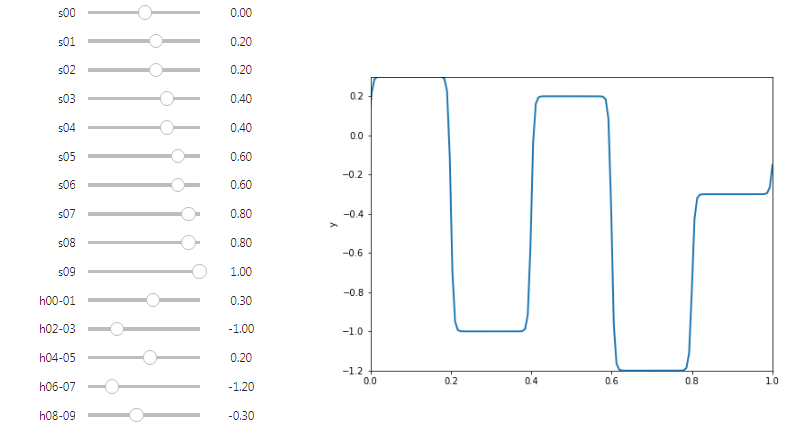
\includegraphics[width=\textwidth,]{pic/wigglyfn21} \par}

